\chapter{Seasonal and interannual variability in bacterial community composition in Antarctic coastal waters}\label{ch:lter}


\chapterdisclaimer{This work was performed in collaboration with Hugh Ducklow, Linda Amaral-Zettler, and Jeremy Rich.\\
\\
Hugh Ducklow and Linda Amaral-Zettler designed and conducted the study with Catherine Luria. Linda Amaral-Zettler and Jeremy Rich contributed sequence data. Catherine Luria analyzed data and wrote this report with guidance from Jeremy Rich. \\
\\
Data included in this chapter also appear in the following publication:\\
Bowman, J. S., Amaral-Zettler, L. A., Rich, J., Luria, C., and Ducklow, H. W. (2016). Bacterial community segmentation facilitates the prediction of ecosystem function along the coast of the western Antarctic Peninsula. \emph{ISMEJ} Accepted.
}


\section{Abstract}

The Western Antarctic Peninsula (WAP) is subject to strong seasonal variability driven by extreme fluctuations in daylength, interannual variability due to large-scale climatic drivers (e.g the Southern Annular Mode), and long-term variability due to rapid climate change in the region that has significantly increased temperatures and reduced sea ice cover over the last several decades. Despite important implications for the movement of materials and energy through the ecosystem, little is known about how these different scales of variability impact bacterial diversity and seasonal succession. Using 16S rRNA gene V6 hypervariable region amplicon sequencing, we assessed bacterial community composition across four Palmer LTER seasons, to identify patterns in seasonal variability and annually recurring successional patterns. While some of the broad trends that we observed were expected (e.g. a midsummer shift toward taxa that respond favorably to phytoplankton blooms), we also observed unexpected, isolated events (e.g. a Colwelliaceae bloom in December 2012) and a surprising degree of interannual variability. Bacterial communities by and large were comprised of a few ``persistent'' operational taxonomic units (OTUs) that were present in most or all samples throughout the time series, and thus, changes in community structures were largely driven by changes in the abundance of just a few taxa. These changes could be linked to both abiotic (day length, serial day, and macronutrients) and biotic (phytoplankton biomass and bacterial production and abundance) factors. Our four-year dataset demonstrates that bacterial community composition may be linked to phytoplankton dynamics, as well as underlying large-scale climatic forces.

\section{Introduction}

The WAP pelagic ecosystem is highly dynamic, with strong seasonal, interannual, and long-term variability. On a seasonal scale, the system oscillates between winters with almost continuous darkness and summers with over 20 hours per day of sunlight. Rapid changes in daylength during the spring transition period drive sea ice retreat and water column stratification. Shoaling of the upper mixed layer allows phytoplankton to overcome light limitation, allowing for intense phytoplankton blooms that support a highly productive food web \citep{Venables2013-me,Smetacek2005-tz}. Bacteria in turn modulate the movement of dissolved organic matter (DOM) produced during phytoplankton blooms through the system via the microbial loop and biological carbon pump \citep{Azam1991-xk,ducklow2001upper}. On an interannual scale, the WAP is subject to strong variability in physical and biological properties that has been linked to Southern Annular Mode (SAM) and El Nino-Southern Oscillation (ENSO) cycles \citep{saba2014winter,Kim2016-dl}. On a decadal scale, the WAP has responded dramatically to climate change; midwinter temperatures have increased by 6\textdegree C and sea ice extent has declined by 40\% over the past few decades \citep{dcddghmmmms12,Schofield2010-jj,Stammerjohn2008-nj}. 

Sea ice is a key driver of variability across multiple temporal scales as the annual advance, retreat and duration of sea ice strongly influence all aspects of the WAP ecosystem including the timing and magnitude of phytoplankton blooms \citep{dsvse12,mddfmss09}. Sea ice enhances primary production through increased water column stratification due to freshening of the surface water, enabling phytoplankton to persist and proliferate in the euphotic layer \citep{Smith1985-lx,Smith1986-en}. Conversely, in years of reduced sea ice, increased wind stress deepens the surface mixed layer, suppressing phytoplankton bloom formation \citep{saba2014winter}. 

Phytoplankton dynamics in turn influence WAP heterotrophic bacteria, which are thought to be primarily regulated by ``bottom up'' factors, particularly the availability of phytoplankton-produced labile DOM \citep{dsvse12,Kirchman2009-sg}. Bacterial production has been extensively studied in the region and is strongly linked to phytoplankton growth \citep{kim2016decedal,luria2016seasonal,dsvse12,Moran2001-ot}. However, there have been relatively few studies of the drivers of WAP bacterial community composition. Studies based on community fingerprinting techniques or on single winter and summer sampling dates report intense seasonality in bacterial and archaeal abundance, diversity, and metabolism \citep{Luria2014-dj,grwddecm12,mpmtbwd98,mg07}. \citet{Luria2014-dj} found similar bacterial communities in winter surface waters (10 m) and summer deep waters (100 m), habitats that share the common feature of reduced light and primary production. Significant changes in community composition concurrent with a summer phytoplankton bloom have also been reported for a single year \citep{luria2016seasonal}. These findings suggest that bacterial community composition responds to the availability of labile organic carbon from phytoplankton. However, the influence of interannual variability in climate modes and sea ice, and hence phytoplankton dynamics, on bacterial succession is unclear.

We surveyed community composition for free-living bacteria over the course of four Palmer Long Term Ecological Research (LTER) seasons (October-March, 2009-2013) and compared our findings to related Palmer LTER environmental datasets. Robust annual patterns have been reported in temperate systems including English Channel \citep{Gilbert2012-ta}, the mid-Atlantic Bight \citep{Nelson2008-fn}, and the coastal waters of Southern California \citep{chow2013temporal,fuhrman2006annually}, and rivers and lakes \citep{Crump2005-kv,Eiler2012-yh}, where temporal changes in community composition recurred on an annual basis with remarkable precision. In contrast, we hypothesized that, given the strong interannual variability in phytoplankton blooms, bacterial community composition would not exhibit strongly recurring annual patterns. Instead, changes in community composition would correspond to variable phytoplankton dynamics. 

\section{Methods}

\subsection{Contextual data collection}

Contextual data, including dissolved nutrients (phosphate, silicate, nitrate and nitrite), particulate organic carbon and nitrogen (POC and PON), chlorophyll \emph{a} (chl \emph{a}), primary production, bacterial abundance, and bacterial production, were collected through the Palmer LTER project. Protocols and curated data are available at \url{http://pal.lternet.edu/data}, as well as through the references cited below. Data from four years were analyzed: October 2009-January 2010 (PAL0910), December 2010-March 2011 (PAL1011), December 2011-March 2012 (PAL1112), and October 2012-March 2013 (PAL1213). Briefly, nutrient and DOC samples were filtered through combusted \SI{0.7}{\micro\meter} glass fiber filters (Whatman, GE Healthcare Life Sciences, Piscataway, NJ) and frozen at -80\textdegree C until analysis on a SEAL AutoAnalyer3 \citep{ducklow_doi_2016a} or Shimadzu TOC analyzer respectively \citep{ducklow_doi_2016c}. POC and PON samples were collected on combusted \SI{0.7}{\micro\meter} glass fiber filters from 0.5-2 L seawater and were frozen at -80\textdegree C until analysis via combustion \citep{ducklow_doi_2016d}. Chl \emph{a} samples, as with POC and PON, were collected on \SI{0.7}{\micro\meter} glass fiber filters from \textasciitilde{}0.5-2 L seawater and were assayed fluorometrically using acetone extracts \citep{schofield_doi_2016}. Primary production was derived from $^{14}$C uptake rates during incubation under in situ light conditions \citep{schofield_doi_2016a}. Bacterial abundance samples were analyzed by flow cytometry following the protocol of \citealt{Gasol2000-mn}, with SYBR\textsuperscript{\textregistered} Green I nucleic acid staining (Invitrogen, Carlsbad, CA) on an Accuri C6 flow cytometer (BD Biosciences, San Jose, CA) \citep{schofield_doi_2016}. Bacterial production was derived from rates of \ce{^3H}-leucine incorporation \citep{ducklow_doi_2016b}.

\subsection{16S rRNA gene library generation}

Samples were collected roughly once per week over the course of four LTER summer seasons using a Go-Flo bottle deployed to a depth of 0 m (2009-2010 and 2010-2011) or 10 m (2011-2012 and 2012-2013) at Arthur Harbor Station B (64\textdegree  46.80' S, 64\textdegree  4.45' W). Microbial communities were collected via vacuum filtration through successive 47-mm diameter \SI{3.0}{\micro\meter} pore-sized TSTP filters (EMD Millipore, Billerica, MA) and \SI{0.2}{\micro\meter} Sterivex{\texttrademark} cartridges (EMD Millipore, Billerica, MA). To preserve DNA, Sterivex cartridges were flooded with sucrose lysis buffer (40 mM EDTA, 50 mM Tris-HCl, 0.75 M sucrose) and were stored at -80\textdegree C until processing. We extracted DNA using a Puregene DNA extraction kit (Qiagen, Valencia, CA) with modifications as previously described \citep{amdh09} and stored extracts at -20\textdegree C until further processing. 

Sequence libraries were generated as in Chapter 3. For each DNA sample, the V6 hypervariable region of the 16S rRNA gene was amplified by polymerase chain reaction (PCR) with custom fusion primers that contained Illumina adaptor and inline barcodes (forward primer) or dedicated indices (reverse primer) as previously described \citep{Eren2013-ob}. Size-selected PCR products were quantified and pooled in equimolar amounts prior to sequencing on one lane of an Illumina HiSeq 1000 cycle paired-end run. 

\subsection{Data analysis}

Low-quality sequences were filtered from the resulting data by discarding reads without 100\% consensus between forward and reverse paired-end sequencing reads \citep{Eren2013-ob}. OTUs were clustered using Qiime (v 1.9.1; \citealt{Caporaso2010-ee}) with open reference OTU picking with the default UCLUST method \citep{Edgar2010-gq}, a minimum cluster size of 2, and a 97\% similarity threshold and were assigned Greengenes taxonomy (version 13\_8; \citealt{McDonald2012-qf}). After removing OTUs classified as chloroplasts, rarefied libraries were produced by randomly down-sampling to 40,000 sequences.

Richness calculations based on the number of OTUs observed in rarefied sequence libraries were compared with non-parametric Chao-Jost richness estimates based on un-rarefied libraries as implemented in the R package \code{iNEXT} \citep{Chao2012-nw, chao2014rarefaction}. Comparisons of observed richness between months (all years pooled) were made using one-way analysis of variance (ANOVA) followed by Tukey's HSD means comparisons using the \code{aov} and \code{TukeyHSD} commands in R \citep{t08}. We assessed the relationship between observed richness and environmental predictors, including serial day, daylength, phosphate, silicate, nitrate and nitrite, chlorophyll \emph{a}, and phaeopigment, using stepwise linear regression with forward-backward variable selection as implemented in the R packages \code{dynlm} and \code{MASS}, minimizing Akaike Information Criteria \citep{venables2002modern,zeileis2016dynlm}. Multivariate models were tested for multicollinearity among predictor variables using \code{vif} in the \code{car} package for R and models with variance inflation factors greater than 5 were discarded \citep{fox2011car}. 

We tested the top 100 OTUs, by mean relative abundance, for significant temporal trends or "seasonality" by fitting linear models, using the \code{lm} function in R, with serial day (days since October 31 within each LTER season) as the independent variable and logit-transformed relative abundance data as the dependent variable (c.f. \citealt{chow2013temporal}). We next divided samples (all years pooled) into either individual months or into two-month periods (October-November, December-January, and February-March) and identified those OTUs that best distinguished each category using a Random Forest supervised machine-learning algorithm as implemented in the R package \code{randomForest} \citep{Breiman2001-og,Liaw2002-zv}. The Random Forest consisted of 5000 classification trees with 77 OTUs evaluated at each node for all categories. 

To examine the relative effects of intra- and interannual variability, samples were grouped by month and by year and changes in community structure were analysed using permutational multivariate analysis of variance (PERMANOVA; \citep{McArdle2001-zn}). The analysis was based on mean group Bray-Curtis dissimilarity using Month and Year as factors and 999 permutations of residuals under a reduced model using \code{adonis}, after testing multivariate homogeneity of group dispersions using \code{betadisper} in the \code{vegan} package for R \citep{Oksanen_2015}. We also performed a Mantel test (Spearman, 999 permutations) comparing our Bray-Curtis dissimilarity matrix to a Euclidean distance matrix based on serial day (days since October 31) using the \code{mantel} function in \code{vegan} \citep{Oksanen_2015}. Beta diversity was visualized by non-metric multidimensional scaling (NMDS) using \code{metaMDS} also in the \code{vegan} package. 

We assessed relationships between environmental variables and OTU relative abundances using linear regression as described above. BIOENV analysis with Bray-Curtis dissimilarity and Spearman correlation \citep{Clarke1993-qq}, as implemented in \code{vegan}, was used to identify the environmental variables that best correlated with bacterial community similarities. Co-occurrence network analyses based on Pearson's correlations revealed relationships among OTUs and between OTUs and external variables (i.e. bacterial production). Networks were generated using the Cytoscape CoNet plugin version 1.1.1.beta and a subnetwork containing OTUs that correlated to bacterial abundance or production or chl \emph{a} ($r > 0.5$) was visualized in Cytoscape version 3.4.0   \citep{faust2012microbial,smobwr}.

All of our sequence data are MIMARKS-compliant \citep{Yilmaz:2011aa} and will be deposited in the NCBI SRA. Copies of the MIMARKS table and chapter figures as well as the R code used for all data analysis and figure production can be accessed at: \url{https://github.com/cmluria/dissertation/Chapter_5_LTER}. 

\section{Results and Discussion}

\subsection{Environmental variability}

The timing and magnitude of phytoplankton growth, based on primary production and chl \emph{a} (Figure \ref{fig:ch4:inorganic_nuts}), and bacterial responses (i.e. production and abundance; Figure \ref{fig:ch4:pp_chl}) varied from year to year. PAL0910 exhibited multiple chl \emph{a} peaks exceeding \SI{10}{\micro\gram \per\liter}, with the most sustained peak in late January coinciding with peaks in bacterial production and abundance. PAL1011 had moderate chl \emph{a} and a sustained period of high bacterial production. In contrast, PAL1112 had consistently low chl \emph{a} and primary and bacterial production. A prominent bloom ({\textgreater}\SI{30}{\micro\gram \per\liter} chl \emph{a}) occurred in early December during PAL1213, with a spike in bacterial production following two weeks later. When all years were pooled, log-log regression of bacterial production versus chl \emph{a} gave a slope of 0.55 ($r^{2} = 0.34$, $p < 0.001$). 

\begin{figure}[htbp] 
\centering 
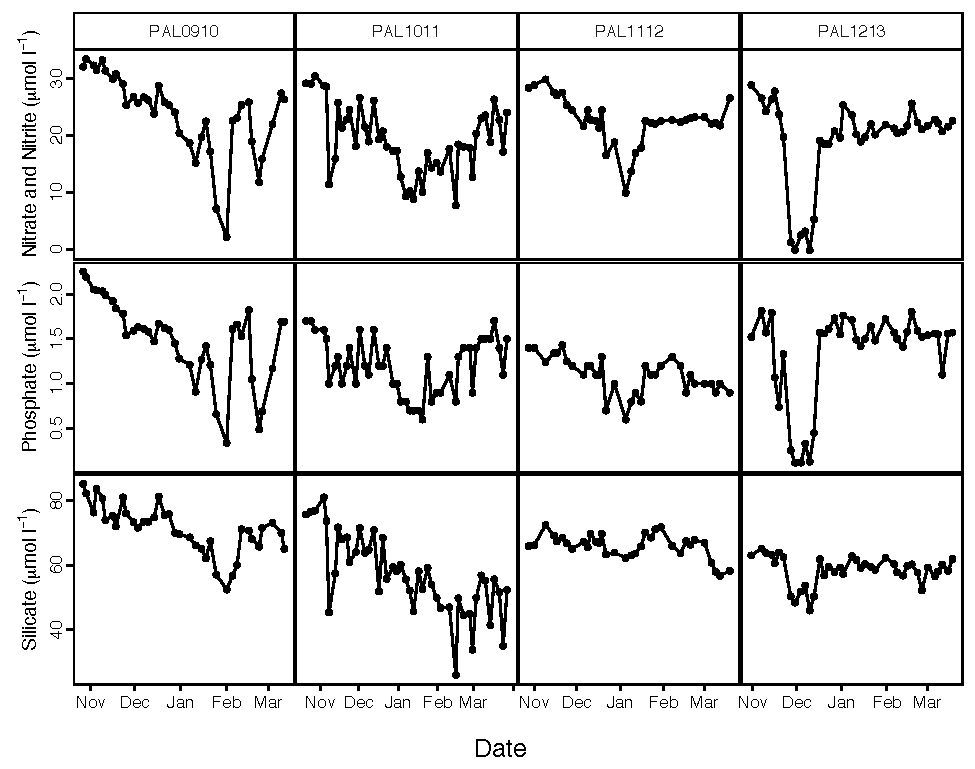
\includegraphics[width=1.0\textwidth]{Chapter_5_LTER/Figures/Figure_1_inorganic_nutrients}
\caption[Inorganic nutrients (nitrate and nitrite, phosphate, and silicate) at Station B across four LTER seasons (PAL0910-PAL1213).]{Inorganic nutrients (nitrate and nitrite, phosphate, and silicate) at Station B (0 m depth) in Arthur Harbor, for four LTER seasons (PAL0910-PAL1213)} 
\label{fig:ch4:inorganic_nuts} 
\end{figure}

\begin{figure}[htbp] 
\centering 
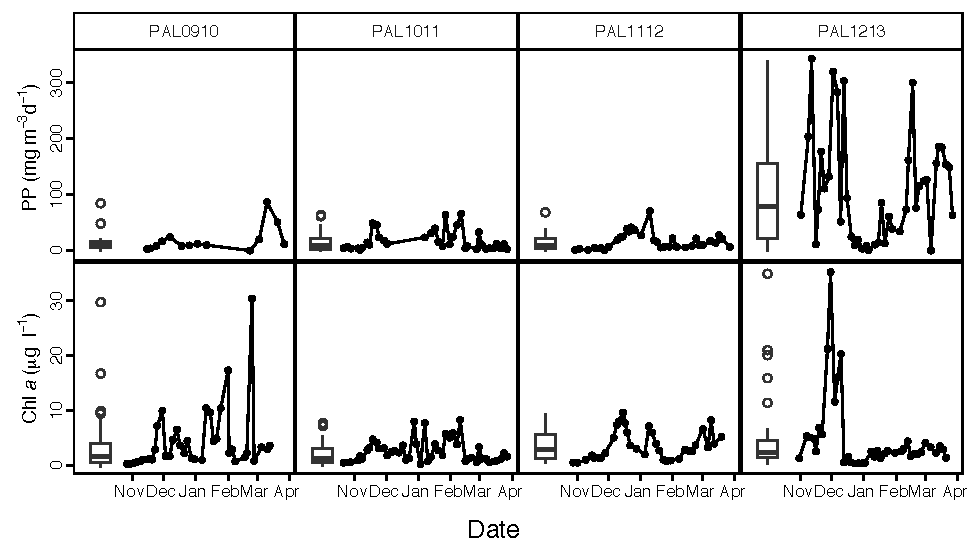
\includegraphics[width=1.0\textwidth]{Chapter_5_LTER/Figures/Figure_2_PP_Chl}
\caption[Phytoplankton dynamics (primary production and chl \emph{a}) at Station B  across four LTER seasons (PAL0910-PAL1213).]{Phytoplankton dynamics (primary production and chl \emph{a}) at Station B (0 m depth) in Arthur Harbor, for four LTER seasons (PAL0910-PAL1213).} 
\label{fig:ch4:pp_chl} 
\end{figure}

Inorganic nutrient drawdown corresponded to periods of increased chl \emph{a} (Figure \ref{fig:ch4:ba_bp}). Nitrate and nitrite and phosphate decreased substantially during the PAL0910 January and PAL1213 December blooms. Some silicate drawdown was evident at these times, as well as during the PAL1011 season when primary production and chl \emph{a} were relatively low. DOC generally oscillated between $45$ and \SI{60}{\micro\mole \per\liter} with no temporal trends evident (Figure \ref{fig:ch4:doc_poc_pon}). POC and PON peaked sharply after a chl \emph{a} peak in PAL0910 (Figure \ref{fig:ch4:doc_poc_pon}), but were surprisingly low during PAL1213, given the magnitude the PAL1213 December phytoplankton bloom. PON was relatively high during the period of sustained bacterial production and silicate drawdown in PAL1011. 

\begin{figure}[ht!] 
\centering 
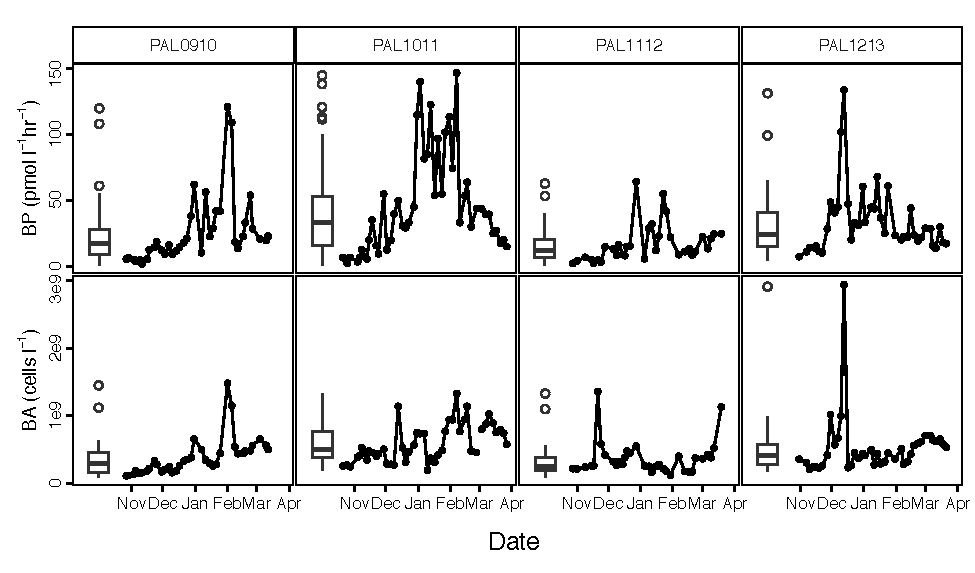
\includegraphics[width=1.0\textwidth]{Chapter_5_LTER/Figures/Figure_3_BA_BP}
\caption[Bacterial dynamics (production and abundance) at Station B across four LTER seasons (PAL0910-PAL1213).]{Bacterial dynamics (production and abundance) at Station B (0 m depth) in Arthur Harbor, for four LTER seasons (PAL0910-PAL1213)} 
\label{fig:ch4:ba_bp} 
\end{figure}

\begin{figure}[ht!] 
\centering 
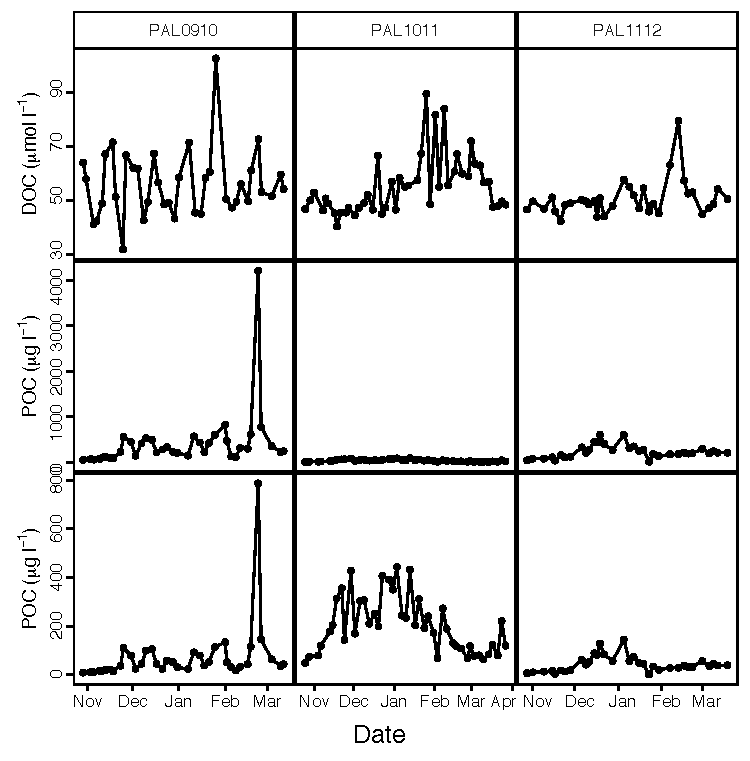
\includegraphics[width=1.0\textwidth]{Chapter_5_LTER/Figures/Figure_4_DOC_POC_PON}
\caption[Dissolved organic carbon and particulate organic carbon and nitrogen at Station B across three LTER seasons (PAL0910-PAL1112).]{Dissolved organic carbon (DOC) and particulate organic carbon (POC) and nitrogen (PON) at Station B (0 m depth) in Arthur Harbor, for three LTER seasons (PAL0910-PAL1112). Data from PAL1213 is not yet available.} 
\label{fig:ch4:doc_poc_pon} 
\end{figure}

The high levels of bacterial production, PON, and silicate drawdown for PAL1011 are surprising given the moderate levels of chl \emph{a} which we observed. This discrepancy was previously noted \citep{kim2016decedal}. \citet{saba2014winter}, pooling data from Station B and Station E and integrating chl \emph{a} and bacteria production for the top 50 m of the water column over almost 25 LTER seasons (PAL8788-PAL1112, December-February only), report a large, positive chl \emph{a} anomaly for PAL0910, a smaller positive anomaly for PAL1011 and a negative anomaly for the PAL1112 season. They attribute the positive anomalies to conditions favored under the negative phase of the SAM: increased winter ice extent and duration, reduced spring/summer winds, and increased water column stratification. Phytoplankton community composition during positive chl \emph{a} anomalies is generally dominated by diatoms, in accordance with the silicate drawdown we observed for PAL1011, whereas the relative abundance of cryptophytes increases in low chl \emph{a} years \citep{saba2014winter}.

\subsection{Persistence and seasonality of individual OTUs} 

Observed richness, or the number of OTUs present in rarefied libraries, varied between 349 and 876 OTUs, with a median of 585 (Figure \ref{fig:ch4:richness}). November had significantly greater richness than December, January, and March ($p < 0.05$) on average, but we did not observe robust seasonal trends, with midsummer richness minima, as previously reported for the WAP, as well as temperate systems \citep{luria2016seasonal,Ladau2013-ro,Gilbert2012-ta}. The lack of winter samples with presumably higher richness may have emphasized otherwise relatively minor fluctuations in richness between our summer samples. Chao-Jost estimated richness, based on un-rarefied libraries, ranged from 1098 to 4163 OTUs with a median of 2347 and was four times greater on average than observed richness based on rarefied libraries (Table \ref{table:ch5:richness}).


\begin{landscape}
\begin{table}[htbp]
\centering
\caption{Observed richness (number of OTUs) for rarefied sequence libraries and Chao-Jost estimated true OTU richness based on un-rarified sequence libraries with 95\% upper and lower confidence intervals (CI).}
\label{table:ch5:richness}
\tiny
\begin{tabular}{@{}lllll@{}}
\toprule
Sample Date & Observed Richness (Rarefied Libraries) & Estimated Richness (Un-rarefied Libraries) & Estimated richness 95\% Lower CI & Estimated richness 95\% Upper CI \\ \midrule
11/3/09     & 876                                    & 4163                                   & 3887                           & 4487                           \\
11/9/09     & 865                                    & 3719                                   & 3406                           & 4094                           \\
11/16/09    & 839                                    & 3423                                   & 3151                            & 3749                           \\
11/18/09    & 812                                    & 3729                                   & 3406                           & 4119                           \\
12/7/09     & 817                                    & 2716                                    & 2508                           & 2969                           \\
12/28/09    & 594                                    & 2846                                   & 2585                           & 3167                           \\
1/11/10     & 466                                    & 2007                                   & 1841                           & 2216                           \\
12/28/10    & 585                                    & 3413                                   & 3099                             & 3795                            \\
1/3/11      & 580                                    & 2547                                   & 2292                           & 2864                           \\
1/10/11     & 689                                    & 2671                                   & 2418                           & 2984                           \\
1/31/11     & 734                                    & 2402                                     & 2153                             & 2713                           \\
2/7/11      & 492                                    & 2590                                   & 2364                           & 2868                           \\
2/15/11     & 757                                    & 2594                                   & 2370                            & 2867                           \\
2/21/11     & 646                                    & 2756                                   & 2516                           & 3050                           \\
3/7/11      & 716                                    & 2781                                    & 2571                           & 3036                           \\
3/14/11     & 677                                    & 2807                                   & 2504                           & 3182                           \\
3/21/11     & 752                                    & 3792                                   & 3495                           & 4146                             \\
3/27/11     & 541                                    & 2873                                   & 2598                           & 3210                           \\
12/6/11     & 542                                    & 2308                                   & 2086                           & 2586                           \\
12/11/11    & 362                                    & 2175                                   & 1949                           & 2465                           \\
12/19/11    & 417                                    & 2176                                   & 1937                           & 2481                           \\
12/28/11    & 392                                    & 2427                                    & 2183                           & 2736                           \\
1/5/12      & 428                                    & 1884                                   & 1713                           & 2102                           \\
1/9/12      & 477                                    & 2503                                   & 2236                          & 2839                           \\
1/30/12     & 714                                    & 3083                                   & 2830                            & 3391                           \\
3/1/12      & 495                                    & 2167                                   & 1957                           & 2432                            \\
3/6/12      & 349                                    & 1329                                   & 1158                           & 1561                           \\
3/12/12     & 419                                    & 2215                                   & 1967                           & 2534                           \\
3/19/12     & 660                                    & 3219                                   & 2925                           & 3578                           \\
10/31/12    & 820                                    & 2904                                   & 2612                           & 3266                             \\
11/7/12     & 805                                    & 1865                                   & 1714                           & 2058                           \\
11/14/12    & 837                                    & 1889                                   & 1667                           & 2177                           \\
11/27/12    & 568                                    & 2015                                   & 1734                             & 2385                           \\
12/4/12     & 422                                    & 1412                                   & 1218                           & 1676                            \\
12/10/12    & 363                                    & 1687                                   & 1510                           & 1916                           \\
12/17/12    & 434                                    & 1394                                   & 1226                           & 1620                           \\
12/23/12    & 862                                    & 2727                                    & 2518                           & 2980                           \\
12/31/12    & 563                                    & 2347                                   & 2026                           & 2760                            \\
1/8/13      & 522                                    & 1672                                   & 1423                            & 2012                           \\
1/14/13     & 440                                    & 2272                                   & 1969                           & 2666                           \\
1/21/13     & 464                                    & 1098                                   & 980                            & 1257                           \\
1/31/13     & 660                                    & 1769                                   & 1569                           & 2028                           \\
2/12/13     & 393                                    & 1397                                   & 1249                           & 1594                           \\
2/18/13     & 665                                    & 1716                                   & 1507                           & 1991                           \\
3/6/13      & 427                                    & 1678                                   & 1492                           & 1922                           \\
3/11/13     & 612                                    & 1191                                    & 1045                           & 1389                           \\
3/18/13     & 843                                    & 1820                                   & 1615                           & 2084                           \\ \bottomrule
\end{tabular}
\end{table}
\end{landscape}

\begin{figure}[htbp] 
\centering 
\includegraphics[width=1.0\textwidth]{Chapter_5_LTER/Figures/Figure_5_richness}
\caption[Bacterial OTU richness at Station B across four LTER seasons (PAL0910-PAL1213).]{Bacterial OTU richness at Station B in Arthur Harbor for four LTER seasons (PAL0910-PAL1213).} 
\label{fig:ch4:richness} 
\end{figure}

Throughout the time series, bacterial communities shared a common core structure. Of the 6143 total OTUs identified, 5482 were ``ephemeral'', appearing in less than 25\% of samples (Figure \ref{fig:ch4:persistence}). Only 144 were ``persistent'', present in more than 75\% of the samples; however, these OTUs accounted for 96.5\% of reads across samples. Fifty-three OTUs were found at every one of the 47 time-points, and these were exceptionally abundant in the sequence data, comprising 88\% of all reads. This pattern, in which a few persistent taxa are also consistently abundant, suggests that many of the changes we observed in community composition reflect variations in the relative abundance of these persistent taxa, as opposed to extinction and colonization processes \citep{Caporaso2011-ec}. Similar findings, in which a few persistent OTUs are also the most abundant, have been reported for the Western English Channel, station ALOHA, California coastal waters, and a freshwater lake \citep{Eiler2011-jl,Eiler2012-yh,Gilbert2009-yi,Caporaso2011-ec,chow2013temporal}. 

\begin{figure}[ht!] 
\centering 
\includegraphics[width=1.0\textwidth]{Chapter_5_LTER/Figures/Figure_6_OTU_persistence}
\caption[Distribution of ``ephemeral'', ``intermittent'', and ``persistent'' OTUs.]{Number of OTUs that occur at different frequencies. Percent frequency was defined as the number of timepoints out of the total timepoints sampled (n=47) that an OTU appeared. OTUs that appeared at less than 25\%, in 25-75\%, or in more than 75\% of the total timepoints were respectively labeled as ``ephemeral'', ``intermittent'', and ``persistent''.} 
\label{fig:ch4:persistence} 
\end{figure}

Forty-three of the top 100 OTUs displayed ``seasonality'', based on a significant correlation with serial day or days since October 31 (all years pooled; $p < 0.05$). These seasonal OTUs accounted for \textasciitilde{}40\% of the community on average. The ten most abundant (by mean relative abundance) of these seasonal OTUs are shown in Figure \ref{fig:ch4:seasonal_otu}. Most but not all OTUs followed a somewhat consistent trajectory; for example, \emph{Polaribacter} (907828) always peaked during the first half of the season, while Flavobacteriaceae (1023473) always declined as the season progressed. 

\begin{figure}[htbp] 
\centering 
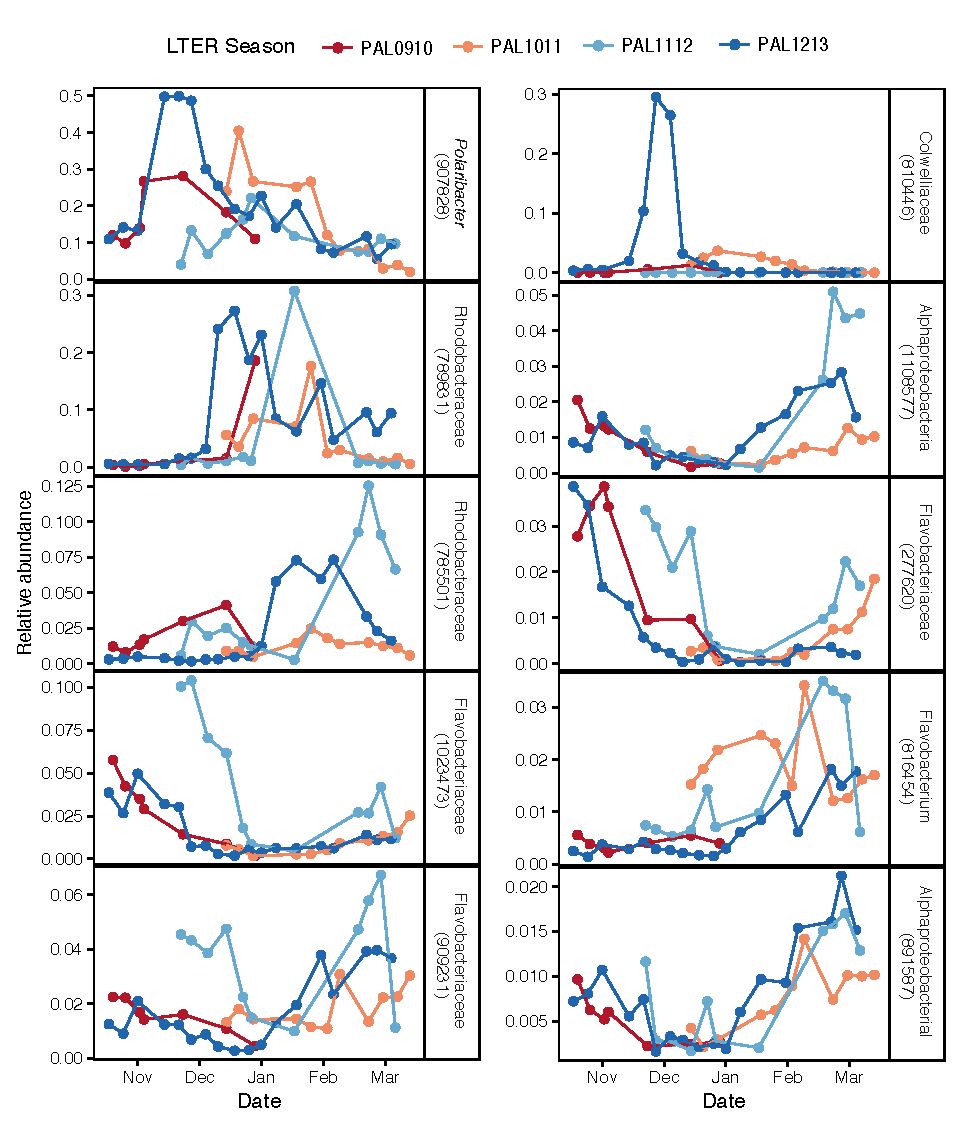
\includegraphics[width=1.0\textwidth]{Chapter_5_LTER/Figures/Figure_7_seasonal_otus}
\caption[Ten most abundant OTUs that displayed ``seasonality''.]{Ten most abundant OTUs (based on average relative abundance) that displayed ``seasonality'', with a significant correlation ($p < 0.05$) between relative abundance and serial day (days since October 31 for each season).} 
\label{fig:ch4:seasonal_otu} 
\end{figure}

\subsection{Seasonal and annual trends in overall community composition}

In general, we did not observe the same sort of robust, recurring annual patterns reported in other marine systems \citep{Gilbert2012-ta,Nelson2008-fn,chow2013temporal,fuhrman2006annually}. Using discriminant function analysis (DFA) to search the taxa that were best able to predict month, \citet{fuhrman2006annually} and \citet{Gilbert2012-ta} were able to assign 80-100\% of samples to the correct month based solely on the distribution and abundance of OTUs, demonstrating interannual repeatability. Similarly, we used Random Forest analysis, a machine learning method of classification, to categorize samples either by individual month or by two-month period (all years pooled): October/November (spring), December/January (mid-summer), and February/March (late summer/early autumn). Unlike DFA, Random Forest analysis does not have any assumptions about the underlying distribution of data and can create models that capture nonlinearities and higher order interactions \citep{Breiman2001-og}. With samples pooled by individual month, Random Forest analysis categorized samples with a 35\% ``out of bag'' error rate. Dividing samples into three two-month categories improved the model, reducing the error rate to 11\%. This suggests that while some repetition in community structure occurs from year to year in the WAP, the patterns are less precise than those reported for other systems. Table \ref{ch4:tab:rf_top} shows the top 20 most predictive OTUs for each two-month period. Some of the predictive OTUs were relatively abundant (e.g. \emph{Polaribacter}), while others were relatively rare but nonetheless predictive of a given time period. Many of the same OTUs were identified as predictive for both the December-January and February-March time periods, while all but one of the OTUs identified for October-November were unique to that category.

\afterpage{
\begin{landscape}
\begin{table}[htbp]
\centering
\caption[Results from Random Forest analysis, identifying OTUs that are predictive of different temporal periods across multiple years.]{Random Forest analysis results. Top 20 predictive OTUs and their nearest taxonomic affiliation for each of three two-month periods (all years pooled): October/November, December/January and February/March.}
\label{ch4:tab:rf_top}
\footnotesize
\begin{tabular}{@{}llllll@{}}
\toprule
\multicolumn{2}{c}{October/November}      & \multicolumn{2}{c}{December/January}        & \multicolumn{2}{c}{February/March}            \\ \midrule
1057746             & Alphaproteobacteria & 1108577             & Alphaproteobacteria   & 1108577             & Alphaproteobacteria     \\
145979              & Acidimicrobiales    & 1110047             & Alteromonadaceae      & 1110047             & Alteromonadaceae        \\
146541              & Cryomorphaceae      & 171966              & Flavobacteriales      & 234515              & Flavobacteriales        \\
158564              & Arctic97B-4         & 234515              & Flavobacteriales      & 3549277             & Rhodobacteraceae        \\
2287192             & Rhizobiales         & 251424              & Rhodobacteraceae      & 3751007             & Flavobacteriales        \\
3223711             & Alphaproteobacteria & 3223711             & Alphaproteobacteria   & 4296166             & \textit{Sediminicola}   \\
339872              & Rhodobacteraceae    & 3751007             & Flavobacteriales      & 541534              & Flavobacteriaceae       \\
4411525             & Rhodospirillaceae   & 396244              & Cryomorphaceae        & 590937              & Rhodobacteraceae        \\
553079              & \textit{Nitrospina} & 4296166             & \textit{Sediminicola} & 594314              & Chromatiales            \\
562219              & Rhodospirillaceae   & 590937              & Rhodobacteraceae      & 741808              & Pelagibacteraceae       \\
567397              & Rhodospirillaceae   & 591094              & Candidatus Portiera   & 752629              & ZD0117                  \\
594314              & Chromatiales        & 752629              & ZD0117                & 792985              & HTCC2089                \\
639731              & \textit{Rubritalea} & 786176              & Rhodobacteraceae      & 816454              & \textit{Flavobacterium} \\
789831              & Rhodobacteraceae    & 792985              & HTCC2089              & 823476              & Alteromonadaceae        \\
830414              & Rhodobacteraceae    & 835045              & Rhodobacteraceae      & 835045              & Rhodobacteraceae        \\
833561              & Pelagibacteraceae   & 891587              & Alphaproteobacteria   & 891587              & Alphaproteobacteria     \\
921366              & \textit{Nitrospina} & 907828              & \textit{Polaribacter} & 907828              & \textit{Polaribacter}   \\
936371              & \textit{Nitrospina} & New.ReferenceOTU481 & Pelagibacteraceae     & New.ReferenceOTU481 & Pelagibacteraceae       \\
New.ReferenceOTU498 & Alphaproteobacteria & New.ReferenceOTU495 & Colwelliaceae         & New.ReferenceOTU495 & Colwelliaceae           \\
New.ReferenceOTU763 & Rhodospirillaceae   & New.ReferenceOTU725 & Unassigned            & New.ReferenceOTU725 & Unassigned              \\ \bottomrule
\end{tabular}
\end{table}
\end{landscape}
}

We also considered how overall community composition varied across different temporal scales. A Mantel test comparing community dissimilarity (Bray-Curtis) and serial day (Euclidean) distance matrices found a statistically significant, but weak relationship between community composition and elapsed time ($r = 0.26$, $p = 0.001$). A PERMANOVA comparison of mean group Bray-Curtis dissimilarities showed that community composition in the months of November ($r = 0.29$), December ($r = 0.67$), January ($r = 0.48$), and March ($r = 0.63$) varied significantly between years (all $p < 0.05$) with the greatest differences observed for December and March. It should be noted that we also observed significant variance in group dispersion among December samples, which violates the implicit assumption of roughly constant within-group multivariate dispersion and could have contributed to the significant PERMANOVA result for that month. Taken together, these results indicate that community composition for a given day or month varies from year to year.

Non-metric multidimensional scaling suggests that while bacterial succession is somewhat predictable from year to year, interannual variability is substantial. (Figure \ref{fig:ch4:nmds}). Some grouping by month across multiple years is evident along NMDS axis 2, indicating a degree of interannual repetition. Spring/early summer (October and November) samples are relatively close to each other, while mid-summer (December, January, and February) samples are more widely scattered. Late summer (March) samples fall at an intermediate point between the two other groups. Some clustering of samples by year is also apparent, especially for PAL1011 and PAL1112, along NMDS axis 1. 

\begin{figure}[htbp] 
\centering 
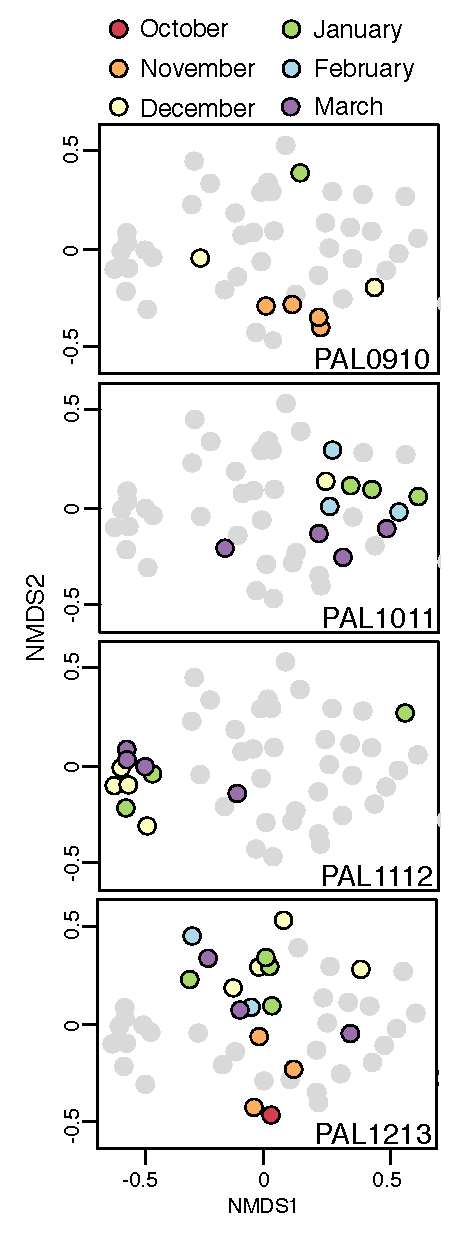
\includegraphics[width=0.5\textwidth]{Chapter_5_LTER/Figures/Figure_8_NMDS}
\caption[Non-metric multidimensional scaling of Bray-Curtis similarity indices based OTU relative abundance.]{Non-metric multidimensional scaling of Bray-Curtis similarity indices of bacterial community composition based OTU relative abundance. A different Palmer LTER season is highlighted in each panel with samples from seasons that are not highlighted shown in grey. Stress = 0.20.} 
\label{fig:ch4:nmds} 
\end{figure}


Finally, we compared pairwise Bray-Curtis similarity versus time elapsed between samples in months (Figure \ref{fig:ch4:bray_curtis}). \citet{chow2013temporal} performed a similar analysis showing annual recurrence as evidenced by Bray-Curtis similarity maxima every 12 months and a slight but significant erosion of community similarity over the course of a decade. We did not observe a similar cyclical pattern in our dataset, nor a significant long term trend. Samples collected even 3 months apart were more similar on average than samples collected exactly 12 months apart, providing little evidence of a repeated annual cycle. However, it is important to note that our time series only spanned the October-March period and did not include the austral winter. Therefore, even ``opposite'' samples, i.e. samples separated by six months, would have been collected in the spring and fall, when communities are relatively similar. The addition of winter samples to our time series would presumably decrease Bray-Curtis similarity between samples collected 6, 18, and 30 months apart and the Bray-Curtis similarity between samples collected exactly 12 months apart would be greater by comparison, perhaps revealing a cyclical pattern. 

\begin{figure}[htbp] 
\centering 
\includegraphics[width=0.8\textwidth]{Chapter_5_LTER/Figures/Figure_9_bray_curtis_over_time}
\caption[Mean pairwise Bray-Curtis community similarity over elapsed time.]{Seasonal and interannual patterns in Bray-Curtis community similarity. Average pairwise community similarity is shown on the Y-axis while the X-axis indicates time lag, the number of months between the communities compared.} 
\label{fig:ch4:bray_curtis} 
\end{figure}

\subsection{Coupling Bacterial Community Structure with Environmental Changes}

Some broad trends in taxonomic succession emerged over the course of several seasons that can be attributed to environmental changes. Among the more prevalent taxa, Pelagibacteraceae, Oceanospirillales, NS9, Rhodospirillales, SAR324, SAR406, and \emph{Nitrospina} tended toward lower relative abundance at mid-summer, while Flavobacteriales, including \emph{Polaribacter} and Rhodobacteraceae, tended toward greater relative abundance at mid-summer (Figure \ref{fig:ch4:taxa} ). The relatively high abundance of SAR406, \emph{Nitrospina}, and SAR324 earlier in the season reflects previous suggestions that chemolithoautotrophy is an important component of bacterial metabolism during the winter \citep{grwddecm12,williams2012metaproteomic,manganelli2009major,wright2014genomic,Spieck2014-sp,Sheik2014-yg}. Certain groups of bacteria (e.g., Flavobacteria and Rhodobacteraceae) have been shown previously to increase in abundance during phytoplankton blooms, while other groups such as \emph{Pelagibacter} are better adapted to non-bloom conditions \citep{williams2013role,Buchan2014-yh,Voget2015-ch}. 

\begin{figure}[ht!] 
\centering 
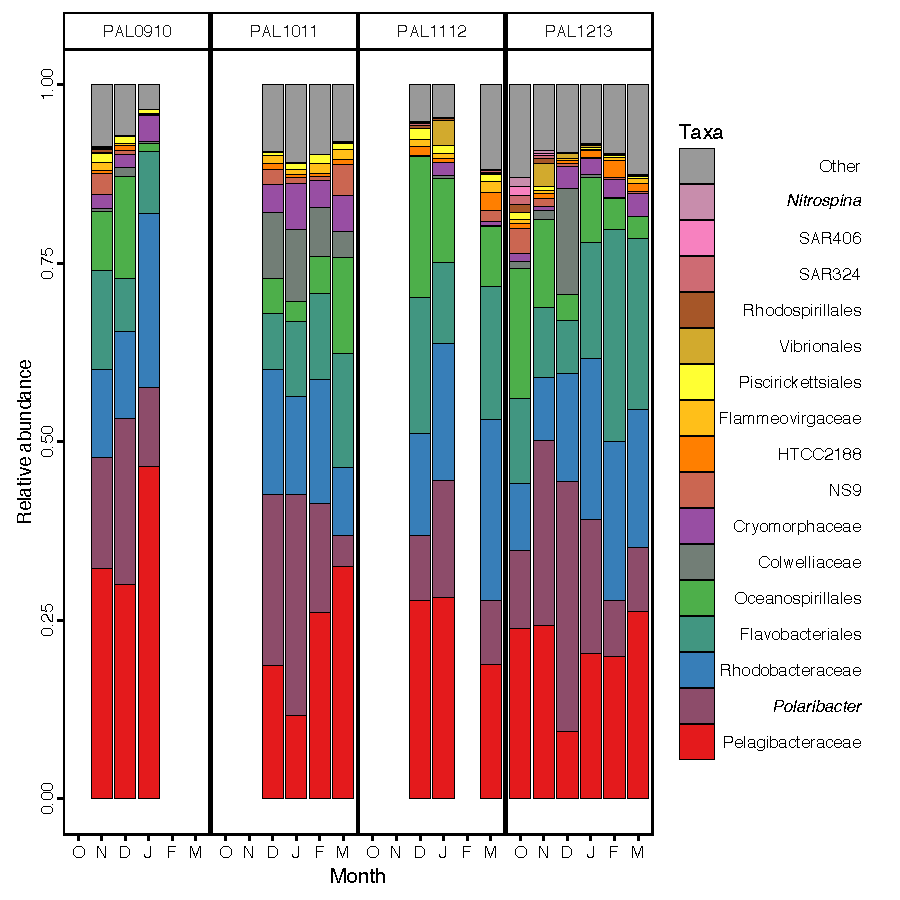
\includegraphics[width=0.8\textwidth]{Chapter_5_LTER/Figures/Figure_10_taxa_barplot}
\caption[Relative abundance of the 16 most common taxa.]{Relative abundance of the 16 most common taxa by mean relative abundance. Mean abundance is shown when more than one library is present for the month shown.} 
\label{fig:ch4:taxa} 
\end{figure}

In contrast to these broad trends, some individual taxa varied widely in abundance from year to year. For example, Colwelliaceae, although relatively rare in most of our samples, was fairly abundant throughout the PAL1011 season, and one Colwelliaceae OTU (810446) ``bloomed'' in December 2012, going from a {\textless}1\% relative abundance to a 30\% relative abundance in the course of one month (Figure \ref{fig:ch4:seasonal_otu} and \ref{fig:ch4:taxa}). Colwelliaceae responded very strongly to diatom-derived DOM during a series of mesocosm experiments (Chapter 4) and their abundance during PAL1011 may reflect the dominance of diatoms during that season and potentially again in December 2012 \citep{saba2014winter}. While PAL0910 was also a high chl \emph{a} year, our DNA time series did not encompass the late January 2010 phytoplankton bloom. During PAL1112, a low chl \emph{a} year, Colwelliaceae had very low relative abundance and we did not observe the midsummer shift between Pelagibacteraceae and \emph{Polaribacter} that occurred in other years.

A stepwise linear regression model based on serial day, daylength, and chl \emph{a} explained 43\% of the variation in richness ($p < 10^{-5}$). Bacterial production was eliminated during variable selection, despite its close association with bacterial community characteristics in our previous study \citep{luria2016seasonal}. Overall community similarities were correlated with a combination of abiotic (day length) and biotic (bacterial production and chl \emph{a}) factors (BIOENV, \emph{rho} = 0.38). BIOENV analysis results were stronger when seasons were considered individually (Table \ref{ch4:tab:bioenv}). For each season, either serial day or day length was an important factor, signaling ``seasonality''. Chl \emph{a} was an important variable in all but one season (PAL1011). Bacterial production was a significant variable in PAL0910, PAL1011, and PAL1213, while bacterial abundance was significant in PAL1112. Surprisingly, one or more macronutrients, which are seldom depleted in the WAP region, were significant for each season. Covariance with other factors may explain the inclusion of nutrients in final BIOENV models. Alternatively, while macronutrients are seldom depleted in the WAP region, they may become more limiting in years with positive chl \emph{a} anomalies \citep{Ducklow2007-ns,saba2014winter}. Overall, these relationships suggest that community structure is linked to both temporal factors with no interannual variability (e.g. day length and serial day) and biotic factors with a high degree of interannual variability (e.g. chl \emph{a} and bacterial production). 

\begin{table}[]
\centering
\caption[Results from BIOENV analysis, linking environmental variables to overall community similarity.]{Results from BIOENV analysis for individual LTER seasons and for all seasons pooled. Only environmental factors for which data was available for almost all dates were considered. These included: serial day, day length, bacterial abundance (BA), bacterial production (BP), phosphate, silicate, nitrate and nitrite, chlorophyll \emph{a} (chl \emph{a}), and phaeopigment.}
\label{ch4:tab:bioenv}
\small
\begin{tabular}{@{}lll@{}}
\toprule
Season     & Environmental factors                                    & BIOENV rho \\ \midrule
All pooled & Day length, BP, chl \emph{a}                             & 0.38       \\
PAL0910    & Serial day, BP, phosphate, silicate, chl \emph{a}, phaeopigment & 0.94       \\
PAL1011    & Serial day, day length, BP, phosphate                    & 0.81       \\
PAL1112    & Day length, BA, nitrate and nitrite, chl \emph{a}        & 0.58       \\
PAL1213    & Serial day, day length, BP, nitrate and nitrite, chl \emph{a}   & 0.66       \\ \bottomrule
\end{tabular}
\end{table}


To explore the relationship between community structure and biotic factors in greater depth, we tested the relationship between relative abundance for the top 100 individual OTUs (by mean relative abundance) and chl \emph{a} and bacterial production. Sixty OTUs correlated significantly with bacterial production, while just 10 correlated significantly with chl \emph{a}, the presumed underlying driver of bacterial production and community structure. A co-occurrence network analysis of individual OTUs associated with key predictive environmental parameters yielded similar results, with several OTUs from the Flavobacteria and Gammaproteobacteria clades associated with bacterial production while just one OTU, classified as \emph{Polaribacter}, was associated directly with chl \emph{a} (Pearson's \emph{r} {\textgreater} 0.5; Figure \ref{fig:ch4:network}). Pelagibacteraceae, which is more competitive under oligotrophic conditions, was negatively associated with bacterial production \citep{Tripp2013-zg}. 

\begin{figure}[ht!] 
\centering 
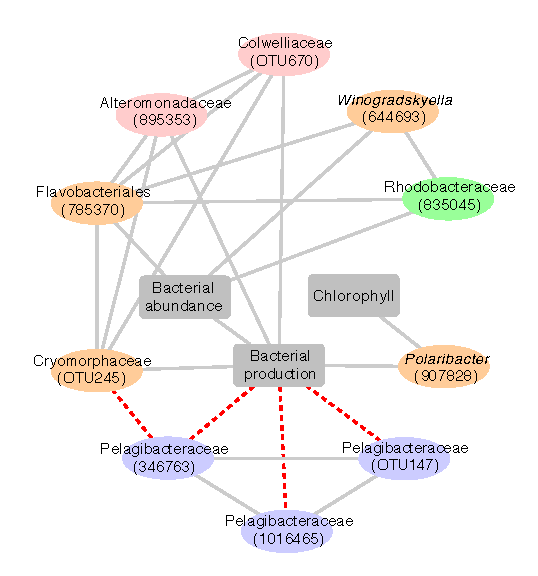
\includegraphics[width=0.8\textwidth]{Chapter_5_LTER/Figures/Figure_11_network_top100otus_minocc0_pearson5_subset_BA_BP_Chl}
\caption[Sub-networks of highly correlated OTUs built around chl a and bacterial production and abundance.]{Sub-networks of highly correlated OTUs built around chl \emph{a} and bacterial production and abundance ($r > 0.5$). Solid, grey lines represent positive correlations; dashed, red lines represent negative correlations. Closest taxonomic identification and reference number (in parentheses) are given for each OTU.} 
\label{fig:ch4:network} 
\end{figure}


While we hypothesized that changes in bacterial community structure would correspond strongly with phytoplankton dynamics, chl \emph{a} and primary production alone did not explain a large fraction of the observed variance in richness and community composition, nor were they significantly linked to many individual OTUs. \citet{kim2016decedal} report considerable interannual variability in the degree of chl \emph{a} control of bacterial production. Furthermore, varying temporal lags between Antarctic phytoplankton blooms and subsequent bacterial responses may confound efforts to model these relationships \citep{billen1991phytoplankton,ducklow2001seasonal,luria2016seasonal}. Such lags are attributed to the need for extracellular hydrolysis of high molecular weight phytoplankton-derived organic matter prior to bacterial uptake \citep{billen1991phytoplankton,ducklow2001seasonal,lancelot1991modelling,kirchman2001glucose}. Additionally, some DOM fractions may only become available through intermediate trophic processes (e.g. zooplankton sloppy feeding or excretion; \citealt{dsvse12}). Therefore, while chl \emph{a} may have been an underlying driver of bacterial community structure, intermediate modulating factors may have obscured its influence. 


We did not consider the influence of ``top-down'' controls, mortality due to bacteriophage induction and predation, which may increase as the season progresses. In the spring, when phytoplankton production and hence DOM availability are low, bacterial community structure is most likely governed by bottom-up controls \citep{bowman2016segmentation}. \citet{Brum2016-ig} report that most phage are in lysogenic phase in the spring and there may be insufficient grazers present to exert substantial top-down control at this point \citep{bowman2016segmentation}. Later in the year, phytoplankton growth may somewhat relieve DOM limitation, while viral abundance and predation may increase \citep{garzio2013microzooplankton,bird1999uncoupling}. As bacterivores and marine viruses disproportionately target rapidly growing cells, top-down controls have the potential to exert a significant control on midsummer bacterial community composition \citep{Fuhrman1993-zk,garzio2013microzooplankton}. 

\section{Conclusions}

Our time series of four LTER seasons encompassed considerable variability in winter/spring physical forcing of phytoplankton dynamics, and subsequently, in bacterial production and biomass, nutrient drawdown, and organic matter availability. Perhaps as a result, we did not observe robust seasonal patterns in OTU richness or strongly recurring annual successional trends for the overall community. Given the interannual variability in phytoplankton growth and a possible mid-season shift between bottom-up and top-down controls, it will be difficult to build robust models for bacterial community composition across multiple years in this dynamic system. However, seasonal trends emerged for individual taxa and OTUs, hinting at diverse ecological niches. The high degree of interannual variability that we observed suggests that multiple years of data encompassing complete SAM and ENSO cycles are needed to capture the range of bacterial community structures that occur in this system.
